
\chapter{Introduction to \texttt{R}}

\section{The \texttt{R} Project for Statistical Computing}

\texttt{R} is a language and environment for statistical computing and graphics. \texttt{R}provides a wide variety of statistical and graphical techniques, and is highly extensible. Among its tools
one can find implemented
\begin{itemize}
	\item linear and nonlinear modelling,
	\item classical statistical tests,
	\item time-series analysis,
	\item classification,
	\item clustering,
	\item ...and many more.
\end{itemize}
One of R's strengths is the ease with which well-designed publication quality plots can be produced.
including mathematical symbols and formulae where needed.
\begin{itemize} \item
	\texttt{R} is a computing software for statistical analysis \item The package is available for all popular operating systems: Windows, Mac or Linux.
	\item It is free!
	\item Everyone (knowledgeable enough) can contribute to the software by
	writing a package.
	\item Packages are available for download through a convenient facility
	\item It is fairly well documented and the documentation is available either
	from the program help menu or from the web-site.
	\item It is the top choice of statistical software among academic statisticians
	but also very popular in industry specially among biostatisticians and
	medical researchers (mostly due to the huge package called
	Bioconductor that is built on the top of \texttt{R}).
	\item It is a powerful tool not only for doing statistics but also all kind of
	scientific programming.
\end{itemize}


\texttt{R} is an integrated suite of software facilities for data manipulation, calculation and graphical display. It
includes
\begin{itemize}
	\item an effective data handling and storage facility,
	\item a suite of operators for calculations on arrays, in particular matrices,
	\item a large, coherent. integrated collection of intermediate tools for data analysis,
	graphical facilities for data analysis and display either on-screen or on hard-copy, and
	\item a well-developed, simple and effective programming language which includes conditionals, loops,
	user-defined recursive functions and input and output facilities.
\end{itemize}

\section{Downloading and Installing \texttt{R}}

\begin{itemize}
	\item \texttt{R} can be downloaded from the CRAN website: http://cran.r-project.org/
	\item You may choose versions for windows, mac and linux.
	\item As per the instructions on the respective pages, you require the ``base" distribution.
	\item Now you can download the installer for latest version of \texttt{R} , version 2.17.
	\item Select the default settings. Once you finish, the \texttt{R} icon should appear on your desktop.
	\item Clicking on this icon will start up the program.
\end{itemize}

\section{Statistical Tables using \texttt{R}}
The following is a fragment of the tables of the values of $F(x)$ for the standard normal (`Z') cumulative distribution function from page 254 of the main textbook.
% Reproduction of Tables

%\begin{center}
%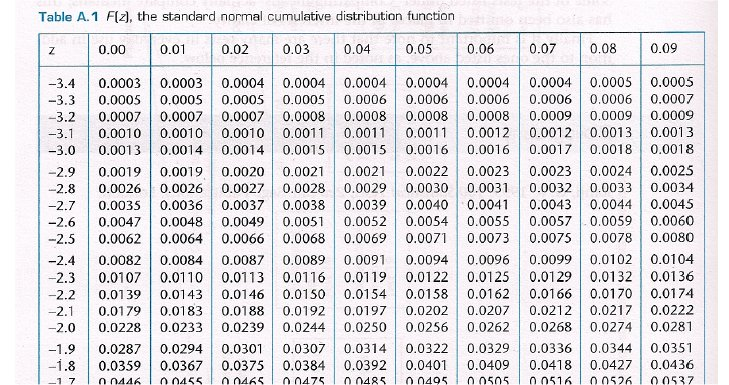
\includegraphics[scale=0.6]{Image6}
%\end{center}
\newpage
\begin{center}
	\line(1,0){250}
\end{center}

\begin{verbatim}
# Segment 1A-1
# Preceding line with the symbol �#� makes it a comment in R
# The following line produce a single value of the standard normal cumulative
# function. It is the value corresponding to the first value in the table

pnorm(-3.4)

#[1] 0.0003369293
#Then the first row of the table

z=seq(-3.4,-3.31,by=0.01)
pnorm(z)

# [1] 0.0003369293 0.0003494631 0.0003624291 0.0003758409 0.0003897124
# [6] 0.0004040578 0.0004188919 0.0004342299 0.0004500872 0.0004664799
# And all values from the table

z=seq(-3.4,3.4,by=0.01)
pnorm(z)

#  [1] 0.0003369293 0.0003494631 0.0003624291 0.0003758409 0.0003897124
#  [6] 0.0004040578 0.0004188919 0.0004342299 0.0004500872 0.0004664799
# [11] 0.0004834241 0.0005009369 0.0005190354 0.0005377374 0.0005570611
# [16] 0.0005770250 0.0005976485 0.0006189511 0.0006409530 0.0006636749
# [21] 0.0006871379 0.0007113640 0.0007363753 0.0007621947 0.0007888457
# [26] 0.0008163523 0.0008447392 0.0008740315 0.0009042552 0.0009354367
# [31] 0.0009676032 0.0010007825 0.0010350030 0.0010702939 0.0011066850

\end{verbatim}
\begin{center}
	\line(1,0){250}
\end{center}
\newpage
There is more than meets the eye in the table. It is not only the table values that can be explored for the
standard normal distribution using \texttt{R}. Recall that the normal
distribution is defined by the density function:
\[
f(z) = \frac{1}{\sqrt(2 \pi)}e^{-Z^2/2}.
\]

The density represents distribution of probability for a random variable associated with it.
The area under the density represents the probability so the that the total area under it is equal to one.
The area accumulated up to certain value $z_o$ represents probability that a corresponding random variable takes
value smaller than z and this probability defines the cumulative distribution function $F(z)$ which is tabularized.


All this can be seen in \texttt{R}. The following code explores various aspects of the standard normal distribution:
\begin{center}
	\line(1,0){250}
\end{center}
\begin{verbatim}

#Plotting the density function of the standard normal variable
z=seq(-3,3,by=0.01)
plot(z,dnorm(z),type='l',col="red",lwd=4)

#Plotting the cumulative distribution function (that one from the table)
plot(z,pnorm(z),type='l',col="red",lwd=4)

\end{verbatim}
\begin{center}
	\line(1,0){250}
\end{center}
\newpage
The \texttt{R} code results in the following plots.
\begin{itemize}
	\item The probability density function.
	\item The cumulative density function.
\end{itemize}
\begin{center}
	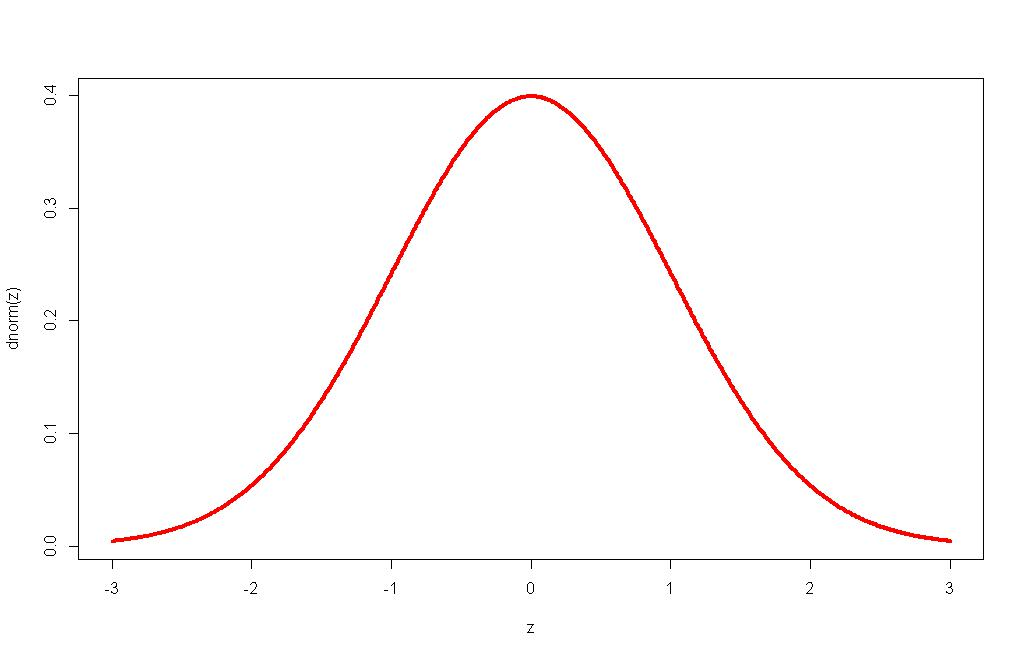
\includegraphics[scale=0.3]{Image7a}
\end{center}
\begin{center}
	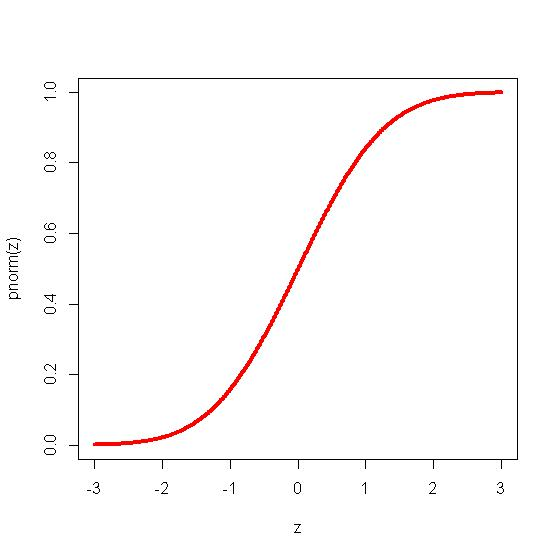
\includegraphics[scale=0.5]{Image7b}
\end{center}
\newpage
\chapter{Introduction to \texttt{R}}

\section{The \texttt{R} Project for Statistical Computing}

\texttt{R} is a language and environment for statistical computing and graphics. \texttt{R}provides a wide variety of statistical and graphical techniques, and is highly extensible. Among its tools
one can find implemented
\begin{itemize}
	\item linear and nonlinear modelling,
	\item classical statistical tests,
	\item time-series analysis,
	\item classification,
	\item clustering,
	\item ...and many more.
\end{itemize}
One of R's strengths is the ease with which well-designed publication quality plots can be produced.
including mathematical symbols and formulae where needed.
\begin{itemize} \item
	\texttt{R} is a computing software for statistical analysis \item The package is available for all popular operating systems: Windows, Mac or Linux.
	\item It is free!
	\item Everyone (knowledgeable enough) can contribute to the software by
	writing a package.
	\item Packages are available for download through a convenient facility
	\item It is fairly well documented and the documentation is available either
	from the program help menu or from the web-site.
	\item It is the top choice of statistical software among academic statisticians
	but also very popular in industry specially among biostatisticians and
	medical researchers (mostly due to the huge package called
	Bioconductor that is built on the top of \texttt{R}).
	\item It is a powerful tool not only for doing statistics but also all kind of
	scientific programming.
\end{itemize}


\texttt{R} is an integrated suite of software facilities for data manipulation, calculation and graphical display. It
includes
\begin{itemize}
	\item an effective data handling and storage facility,
	\item a suite of operators for calculations on arrays, in particular matrices,
	\item a large, coherent. integrated collection of intermediate tools for data analysis,
	graphical facilities for data analysis and display either on-screen or on hard-copy, and
	\item a well-developed, simple and effective programming language which includes conditionals, loops,
	user-defined recursive functions and input and output facilities.
\end{itemize}

\section{Downloading and Installing \texttt{R}}

\begin{itemize}
	\item \texttt{R} can be downloaded from the CRAN website: http://cran.r-project.org/
	\item You may choose versions for windows, mac and linux.
	\item As per the instructions on the respective pages, you require the ``base" distribution.
	\item Now you can download the installer for latest version of \texttt{R} , version 2.17.
	\item Select the default settings. Once you finish, the \texttt{R} icon should appear on your desktop.
	\item Clicking on this icon will start up the program.
\end{itemize}

\section{Statistical Tables using \texttt{R}}
The following is a fragment of the tables of the values of $F(x)$ for the standard normal (`Z') cumulative distribution function from page 254 of the main textbook.
% Reproduction of Tables

%\begin{center}
%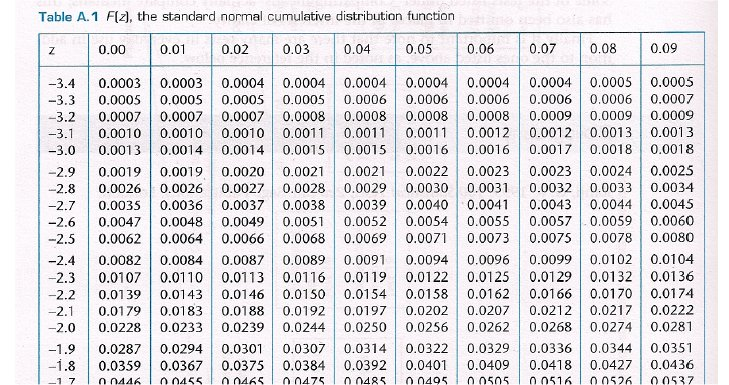
\includegraphics[scale=0.6]{Image6}
%\end{center}
\newpage
\begin{center}
	\line(1,0){250}
\end{center}

\begin{verbatim}
# Segment 1A-1
# Preceding line with the symbol �#� makes it a comment in R
# The following line produce a single value of the standard normal cumulative
# function. It is the value corresponding to the first value in the table

pnorm(-3.4)

#[1] 0.0003369293
#Then the first row of the table

z=seq(-3.4,-3.31,by=0.01)
pnorm(z)

# [1] 0.0003369293 0.0003494631 0.0003624291 0.0003758409 0.0003897124
# [6] 0.0004040578 0.0004188919 0.0004342299 0.0004500872 0.0004664799
# And all values from the table

z=seq(-3.4,3.4,by=0.01)
pnorm(z)

#  [1] 0.0003369293 0.0003494631 0.0003624291 0.0003758409 0.0003897124
#  [6] 0.0004040578 0.0004188919 0.0004342299 0.0004500872 0.0004664799
# [11] 0.0004834241 0.0005009369 0.0005190354 0.0005377374 0.0005570611
# [16] 0.0005770250 0.0005976485 0.0006189511 0.0006409530 0.0006636749
# [21] 0.0006871379 0.0007113640 0.0007363753 0.0007621947 0.0007888457
# [26] 0.0008163523 0.0008447392 0.0008740315 0.0009042552 0.0009354367
# [31] 0.0009676032 0.0010007825 0.0010350030 0.0010702939 0.0011066850

\end{verbatim}
\begin{center}
	\line(1,0){250}
\end{center}
\newpage
There is more than meets the eye in the table. It is not only the table values that can be explored for the
standard normal distribution using \texttt{R}. Recall that the normal
distribution is defined by the density function:
\[
f(z) = \frac{1}{\sqrt(2 \pi)}e^{-Z^2/2}.
\]

The density represents distribution of probability for a random variable associated with it.
The area under the density represents the probability so the that the total area under it is equal to one.
The area accumulated up to certain value $z_o$ represents probability that a corresponding random variable takes
value smaller than z and this probability defines the cumulative distribution function $F(z)$ which is tabularized.


All this can be seen in \texttt{R}. The following code explores various aspects of the standard normal distribution:
\begin{center}
	\line(1,0){250}
\end{center}
\begin{verbatim}

#Plotting the density function of the standard normal variable
z=seq(-3,3,by=0.01)
plot(z,dnorm(z),type='l',col="red",lwd=4)

#Plotting the cumulative distribution function (that one from the table)
plot(z,pnorm(z),type='l',col="red",lwd=4)

\end{verbatim}
\begin{center}
	\line(1,0){250}
\end{center}
\newpage
The \texttt{R} code results in the following plots.
\begin{itemize}
	\item The probability density function.
	\item The cumulative density function.
\end{itemize}
\begin{center}
	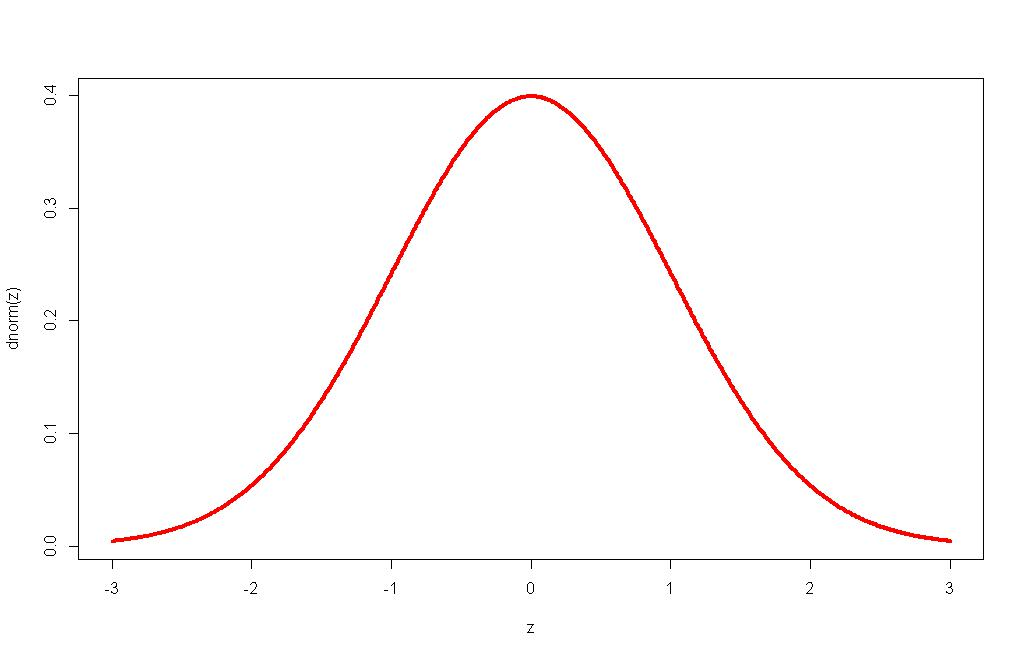
\includegraphics[scale=0.3]{Image7a}
\end{center}
\begin{center}
	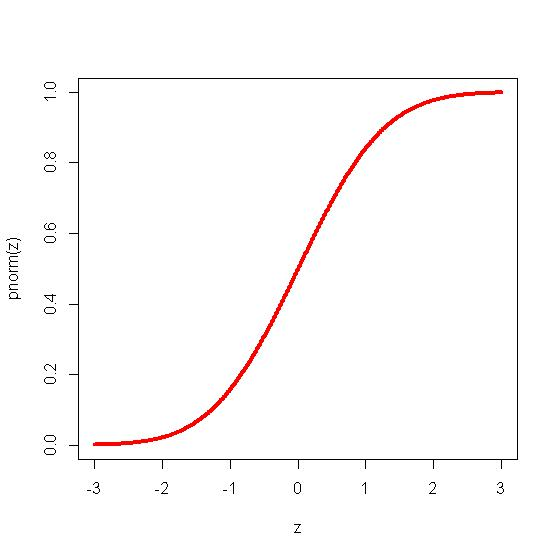
\includegraphics[scale=0.5]{Image7b}
\end{center}
\newpage